  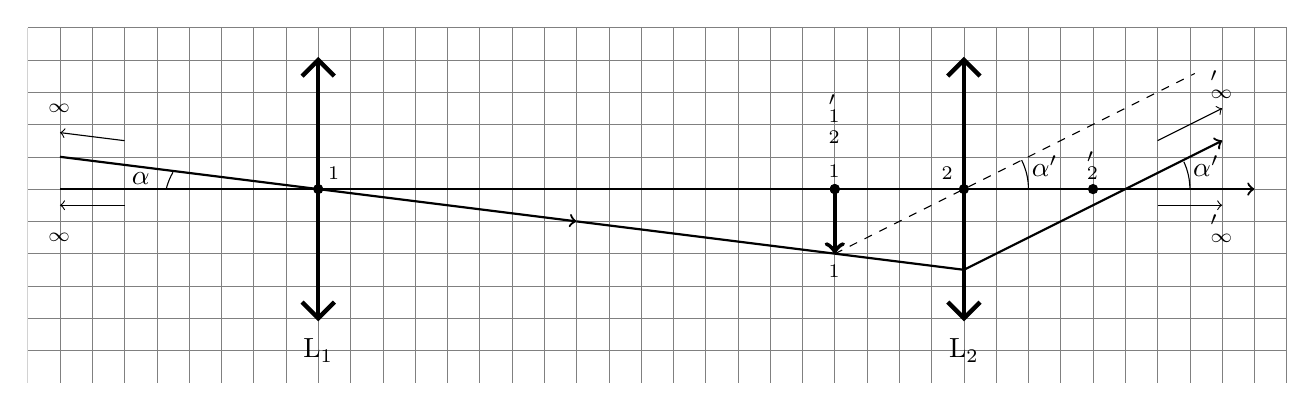
\begin{tikzpicture}[scale=0.82]
    \clip (-4.5,-3) rectangle (15,2.5) ; %Les dimensions de l'image
    \draw [help lines] (-4.5,-3) grid [step=0.5] (15,2.5) ; %% Le quadrillage
    \draw [->,thick] (-4,0) -- (14.5,0) ; %% L'axe optique
    
    \draw [ultra thick] (0,-2) -- (0,2)  ; %% Le corps de la lentille L1
    
    \draw [ultra thick] (-0.25,-1.75) -- (0,-2) -- (0.25,-1.75)
                         (-0.25,1.75) -- (0,2) -- (0.25,1.75) ;                    %La lentille L1
                         
     \draw [ultra thick] (10,-2) -- (10,2)  ; %% Le corps de la lentille L2 
    
    \draw [ultra thick] (9.75,-1.75) -- (10,-2) -- (10.25,-1.75)
                         (9.75,1.75) -- (10,2) -- (10.25,1.75) ;                    %La lentille L2

    \filldraw [black] (0,0) circle (2pt) node [above right] {$\ptO_1$} ;  %Le centre optique de L1
    \filldraw [black] (8,0) circle (2pt) node at (8,1.25) {$\ptF'_1$}; %Le foyer image de L1
    
    \filldraw [black] (10,0) circle (2pt) node [above left] {$\ptO_2$} ;  %Le centre optique de L2
    \filldraw [black] (8.0,0) circle (2pt) node at (8,0.8) {$\ptF_2$} ; %Le foyer objet de L2
    \filldraw [black] (12.0,0) circle (2pt) node[above]{$\ptF'_2$} ; %Le foyer image de L2
    
      \draw [->,ultra thick] (8,0) node [above] {$\ptA_1$} -- (8,-1.0) node [below] {$\ptB_1$} ;     %L'image intermédiaire
     
     \draw [-,thick] (-4,0.5) -- (0,0) ; %% Rayon lumineux 
     \draw [->,thick] (0,0) -- (4,-0.5) ; %% Rayon lumineux
     \draw [-,thick] (4,-0.5) -- (8,-1) ; %% Rayon lumineux
     \draw [-,thick] (8,-1) -- (10,-1.25) ; %% Rayon lumineux  
     \draw [->,thick] (10,-1.25) -- (14,0.75) ; %% Rayon lumineux  
     \draw[dashed,shift={(10,0)}](-153.4:{sqrt(5)})--(26.6:4);% Rayon annexe pour justifier la construction
     
     \draw node at (0,-2.5) {$\mathrm{L_1}$} ; %Légende L1
     \draw node at (10,-2.5) {$\mathrm{L_2}$} ; %Légende L2
     
   \draw (-2.25,0.26) arc (150:165:1) ;
   \draw node at (-2.75,0.17) {$\alpha$} ; %Repérage angle alpha
   
   \draw (13.5,0) arc (0:25:1) ;
   \draw node at (13.75,0.35) {$\alpha'$} ; %Repérage angle alpha'
  
   \draw (11,0) arc (0:26.6:1) ;
   \draw node at (11.25,0.35) {$\alpha'$} ; %Repérage angle alpha'

 
   \draw node at (-4,1.25) {$\ptB_{\infty}$} ; %Objet B
   \draw [->,thin] (-3,0.75) -- (-4,0.875) ; %% Direction objet B
   
%   \draw node at (13.5,1.5) {$\ptB'_{\infty}$} ; %Image finale B'
   \draw [->,thin] (13,0.75) -- (14,1.25) node[above]{$\ptB'_{\infty}$}; %% Direction image B'
   
   \draw node at (-4,-0.75) {$\ptA_{\infty}$} ; %Objet A
   \draw [->,thin] (-3,-0.25) -- (-4,-0.25)  ; %% Direction objet A
   
%   \draw node at (13.5,-0.75) {$\ptA'_{\infty}$} ; %Image finale A'
   \draw [->,thin] (13,-0.25) -- (14,-0.25) node[below]{$\ptA'_{\infty}$}; %% Direction image A'
      
  \end{tikzpicture}